\section{The GraphBLAS}
\label{sec:math}

%%  <<< Self Plagiarism Warning >>>>
%% The text from here to the end of the operations table was lifted from our
%% GABB paper where we introduced the C API
Consider a graph represented as an $n$-by-$n$ adjacency matrix $\matrix{A}$,
where $A_{ij}$ is the weight of the edge from vertex $i$ to vertex $j$,
and a second $k$-by-$n$ matrix $\matrix{B}$ representing a subset (of size k) of the vertices
in the graph, such that $B_{ji}$ is $1$ if the $j$th element of the subset is vertex $i$
(and all other elements of $\matrix{B}$ are 0).  The traditional matrix
product $\matrix{B} \times \matrix{A}$ over real arithmetic of these two matrices returns 
the cost based on the edge weights of reaching the set of vertices
adjacent to the vertices in $\matrix{B}$.  This fundamental operation can be
used to construct a wide range of graph algorithms.

We extend the range of graph operations by keeping the basic
pattern of a matrix-matrix multiplication, but varying
the operators and the interpretation of the values in the matrices (the \emph{domain}).
By carefully choosing operators and the domain, we control the
relation between matrix operations familiar in linear algebra and graph operations, thereby enabling
composable graph algorithms.

In addition to matrix multiplication, the GraphBLAS math specification defines
a range of additional operations over matrices and vectors.  These are summarized in Table~\ref{Tab:GraphBLASOps}.

\begin{table}[h]
\hrule
\begin{center}
\caption{A mathematical overview of the fundamental GraphBLAS operations supported
in the specification. $\matrix{A}$, $\matrix{B}$, and $\matrix{C}$ are GraphBLAS matrices; 
$\vector{u}$, $\vector{v}$, and $\vector{w}$ are GraphBLAS vectors; $i$ and $j$ are single indices;
$\mathbf{i}$ and $\mathbf{j}$ are arrays of indices;
$\oplus$ and $\otimes$ are arbitrary element-wise operators; the element-wise $\odot$
operator is used for the optional accumulation with the output GraphBLAS object where 
$x~\odot\hspace{-0.11cm}= y$ implies $x = x \odot y$; and $F_u()$ is a unary function.
Although not shown here, the input 
matrices $\matrix{A}$ and $\matrix{B}$ may be selected for transposition prior to 
the operation, and masks can be used to control which values are written to the output GraphBLAS object.
\label{Tab:GraphBLASOps}}
\newcommand{\odotequals}{~\odot\hspace{-0.09cm}=\hspace{-0.2cm}}
\begin{tabular}{l|rl}
{\sf Operation name} & \multicolumn{2}{c}{Mathematical description}  \\
\hline
{\sf mxm}          & $\matrix{C}$    $\odotequals$ & $\matrix{A} \oplus.\otimes \matrix{B}$ \\
{\sf mxv}          & $\vector{w}$    $\odotequals$ & $\matrix{A} \oplus.\otimes \vector{v}$ \\
{\sf vxm}          & $\vector{w}^T$  $\odotequals$ & $\vector{v}^T \oplus.\otimes \matrix{A}$  \\
{\sf eWiseMult}    & $\matrix{C}$    $\odotequals$ & $\matrix{A} \otimes \matrix{B}$ \\
                   & $\vector{w}$    $\odotequals$ & $\vector{u} \otimes \vector{v}$ \\
{\sf eWiseAdd}     & $\matrix{C}$    $\odotequals$ & $\matrix{A} \oplus \matrix{B}$ \\
                   & $\vector{w}$    $\odotequals$ & $\vector{u} \oplus \vector{v}$ \\
{\sf reduce} (row) & $\vector{w}$    $\odotequals$ & $\bigoplus_j\matrix{A}(:,j)$  \\
{\sf apply}        & $\matrix{C}$    $\odotequals$ & $F_u(\matrix{A})$ \\
                   & $\vector{w}$    $\odotequals$ & $F_u(\vector{u})$ \\
{\sf transpose}    & $\matrix{C}$    $\odotequals$ & $\matrix{A}^T$ \\
{\sf extract}      & $\matrix{C}$    $\odotequals$ & $\matrix{A}(\vector{i},\vector{j})$ \\
                   & $\vector{w}$    $\odotequals$ & $\vector{u}(\vector{i})$ \\
{\sf assign}       & $\matrix{C}(\vector{i},\vector{j})$  $\odotequals$ &  $\matrix{A}$ \\
                   & $\vector{w}(\vector{i})$  $\odotequals$ & $\vector{u}$ 
\end{tabular}

\end{center}
\hrule
\end{table}

%% << end of self-plagrism >>>

In mapping the GraphBLAS as a set of mathematical operators onto the C programming language
we made a number of fundamental choices~\cite{cspec}.  First, the core data structures required
to represent the objects defined by the GraphBLAS are opaque.   The GraphBLAS API defines a 
contract with the programmer for how these objects will be used, but the implementations and underlying
data structures are left to the implementation.  This opaqueness is critical if the API is to serve diverse hardware
ranging from CPUs to GPUs to specialized graph hardware. Second, we defined a non-blocking  
execution model that allows lazy evaluation.  Ultimately, to optimize sparse linear algebra software we need
to aggressively fuse operations and even restructure algorithms.  This requirement meant that we had to 
carefully define when results from a sequence of GraphBLAS operations must be materialized.

Since the release of the GraphBLAS specification, several implementations of the GraphBLAS have been
developed. These are briefly described below.

% SuiteSparse GraphBLAS:

\subsection{SuiteSparse:GraphBLAS}

SuiteSparse:GraphBLAS is the first full implementation of the GraphBLAS
standard, first released in November of 2017.
It is available at \url{http://suitesparse.com} \cite{Davis19}.

The design of a GraphBLAS library is flexible, because its data structures are
opaque to the user.  SuiteSparse:GraphBLAS uses a compressed-sparse vector
data structure, in four different forms.  A matrix can be stored in
row-major order (CSR), or column-major order (CSC).  Each sparse vector
consists of a sorted list of indices, and the corresponding numerical values.
The sparse vectors are packed together into two arrays, and another ``pointer
array'' (of size equal to the dimension of the matrix, say $n$) keeps track of
where each row (or column) starts.  The memory taken is $O(n+e)$ for a CSR
matrix with $n$ rows or a CSC matrix with $n$ columns, and with $e$ entries.
Most graphs have $e=O(n)$ entries, but some graphs (and in particular,
subgraphs) can be {\em hypersparse} \cite{BulucGilbert08}, with $e << n$.  In
the hypersparse form, the pointer array itself becomes sparse, and empty
vectors take no space at all.  The space is reduced to $O(e)$, so that
matrices with enormous dimensions can be created, as long as $e << n$.
SuiteSparse:GraphBLAS exploits hypersparsity automatically, and all
methods can operate on all four matrix formats in any combination.

The ability to incrementally modify a graph is critical in many applications.
GraphBLAS includes two operations that can make small incremental changes to a
graph/matrix:  namely \verb'GrB_setElement' and \verb'GrB_assign'.  It would be
exceedingly slow to insert or delete a single entry in a CSR or CSC format,
taking $O(n+e)$ time {\bf per entry} inserted or deleted.  Instead, the
non-blocking aspect of GraphBLAS is exploited.  Fast deletion of entries is
handled by creating {\em zombies}, which are entries tagged for later deletion.
Fast insertion is handled with {\em pending tuples}, which is a separate
unordered list of $(i,j,a_{ij})$ for each new entry.  When a matrix operation
occurs (such as matrix multiply), all zombies are killed and all pending tuples
are assembled, in a single $O(n+ e + p \log p)$ step (for $p$ pending tuples),
or $O(e +p \log p)$ in the hypersparse case.  As a result, it is just as fast
to use a sequence of $e$ \verb'GrB_setElement' operations to build a matrix, as
it is to create an array of $e$ tuples and use \verb'GrB_build'.  Internally,
SuiteSparse:GraphBLAS is building the list itself, for the user, and then does
a \verb'GrB_build' when the matrix needs to be completed.

To enable high-performance matrix-matrix multiply, a code generation mechanism
is used to build functions for each semiring that can be created with built-in
operators.  The functions can rely on Gustavson's method \cite{Gustavson78}, a
dot product method, and a heap-based method \cite{sisc3dspgemm}, all with
masked variants.  A current prototype of the package adds an early exit
mechanism for the MIN, MAX, OR, and AND monoids, where a dot product can
terminate as soon as a terminal value is found in the result (\verb'true' for
OR, for example).  This will enable a fast direction-optimizing BFS
\cite{Beamer:2012:DOB} to be written in GraphBLAS.  The ``pull'' is a dot
product, and the ``push'' a saxpy-based operation (Gustavson's or the heap
method).

Since its creation was commissioned as the GraphBLAS reference implementation,
testing is a vital component to the package.  In SuiteSparse:GraphBLAS, each
GraphBLAS operation was written twice: once in high-performance algorithms in
C, and again in a very simple and short MATLAB script, using dense matrices
with the required type.  The pattern in the MATLAB version is held as a
separate Boolean matrix.  For example, \verb'GrB_assign' requires about 3,908
lines of C (not counting comments), but only 161 lines in MATLAB. Of those 161
lines, 33 are for error-checking that do not need to be considered when
determining conformance to the spec.  The MATLAB functions are not intended to
be fast.  Instead, they exactly mimic the GraphBLAS API Specification, line by
line, so they can be visually inspected for conformance to the spec.  For
example, matrix multiply is written with a brute-force triply-nested \verb'for'
loop.  Then, to test the package, each computation is done both in
SuiteSparse:GraphBLAS (via a MATLAB interface) and in the MATLAB mimic.  The
tests pass only if the results are identical in both value and pattern (even
with identical floating-point roundoff error, in most cases).

The current release is single-threaded, but an OpenMP implementation is in
progress.  SuiteSparse:GraphBLAS appears in Debian and Ubuntu Linux distros,
and has been released as part of the RedisGraph database module of the Redis
database systems, by RedisLabs, Inc. \cite{redisgraph}.



% IBM GraphBLAS:
\subsection{IBM GraphBLAS}

\newcommand{\code}[1]{{\tt #1}}

The IBM GraphBLAS implementation was announced at IPDPS 2018 and made
available at \code{https://github.com/IBM/ibmgraphblas}, fulfilling
the GraphBLAS C API requirement of two conforming implementations,
and promoting that specification from \emph{provisional} to
\emph{definitive}. The approach adopted by the development team was
heavily influenced by their experience with IBM's Graph Programming
Interface~\cite{gpi2016,GPI}.

Among the various objectives of the IBM implementation, we note the
desire to experiment with an implementation that allows multiple data
representations and a layered approach to algorithms, keeping a GraphBLAS
API layer on top of a more fundamental \emph{back-end} layer that performs
the heavy computation.

Use and operation of the IBM GraphBLAS is straightforward.
The application programmer has access to a C11-compliant include
file (\code{GraphBLAS.h}) that defines the API according to the
specification. This include file exposes nothing of the internals of
the run-time. The run-time itself is written in C++ and packaged as a
library (\code{libibmgraphblas.so}) with C language bindings.  The choice
of C++ as the implementation language has led to a simple and concise
specification-compliant implementation.

One of the jobs of the \code{GraphBLAS.h} include file is to
convert the polymorphic version of the API into the nonpolymorphic
one. The nonpolymorphic methods are then directly supported by the
library. Conversion of the polymorphic interface is accomplished through
standard C preprocessor features, primarily in supporting number of
arguments polymorphism, in combination with the standard C11 language
\code{\_Generic} construct to support type polymorphism.

As previously mentioned, the IBM GraphBLAS library is implemented in
C++. The API methods are declared to have a C interface, so that C user
programs can bind to them as specified. Objects internal to the library
are declared as C++ classes, with member methods doing the actual work.
We want to emphasize that this is a C++ implementation of a C API, and
not an API for GraphBLAS that exploits C++ features, as other efforts
are pursuing~\cite{gbtl-github} (see \autoref{sec:gbtl}).

The contents of a GraphBLAS vector object are implemented using standard
C++ containers.  An unordered set of indices (\code{uset<GrB\_Index>})
is used to represent the structure of the vector, while an unordered
map of indices to pointers (\code{umap<GrB\_Index,void*>}) represents
the elements.  (Currently, \code{uset} and \code{umap} are just renames
for the \code{std::unordered\_set} and \code{std::unordered\_map} standard
containers of C++, but one could use more specialized implementations.)

Similarly, the contents of a matrix are represented both as a standard
C++ container vector of rows and a standard C++ container vector of
columns. Accessor methods enforce consistency of both representations.

In the current IBM GraphBLAS, all methods are fully blocking. That is,
the methods return only after all computations are fully performed (or
an error is detected).  Since the GraphBLAS nonblocking mode allows for
deferred execution but does not require it, this behavior complies with
the specification.

We finish this brief overview of the IBM GraphBLAS with a discussion
of error handling, as we believe it reflects an important aspect of the
interoperability between a C API and a C++ implementation.  The GraphBLAS
C API defines two kinds of errors: API errors and execution errors.
API errors reflect incorrect usage of the API (for example, passing
parameters that are not valid or consistent). Execution errors indicate
that something went wrong during the actual execution of a method,
and can be caused either by programmer error or by environment issues
(for example, not enough memory).

In the IBM GraphBLAS run-time, API errors are detected through
explicit checks in the implementation of each method in the API layer
(the \emph{front-end}).  Execution errors, on the other hand, occur
inside the member methods of the various objects internal to the library
(the \emph{back-end}).  Those methods, following standard C++ practice,
use exceptions to signal an error. To transform those exceptions into
proper GraphBLAS C API return codes, the body of each GraphBLAS API
method is wrapped by a \code{try}/\code{catch} block, which then returns
the GraphBLAS execution error code corresponding to the caught exception.


% GBTL: GraphBLAS Template Library
\subsection{GBTL: GraphBLAS Template Library}
\label{sec:gbtl}

The first version of the GraphBLAS Template Library (GBTL) was written in C++ 
when the GraphBLAS C API project was just beginning.  It was used, in part, 
to study early ideas under discussion in the specification process and was released as a proof of concept 
prior to the finalization of the GraphBLAS API Specification \cite{gbtl-cuda16, McMillan2016}. With the 
release of the GraphBLAS C API Specification~\cite{cspec} in 2017, GBTL was updated to conform to 
the mathematical behavior defined by the specification and released as version 2.0~\cite{gbtl-github}.  
Unlike the C API Specification, GBTL is written in C++ and makes judicious use of templates to 
make the generic aspects of the GraphBLAS specification easier to implement and 
more natural for the C++ programming language. When the GraphBLAS language committee
starts its work on the C++ language binding to the GraphBLAS, GBTL will be submitted as a 
proposed starting point for the discussion.

 
Central to GBTL's design is the concept of a separation of concerns between 
implementation of algorithms written in terms of the GraphBLAS primitives  
and the implementation of those primitives on a targeted hardware platform.   
This separation of concerns is defined by the GraphBLAS API Specification as
illustrated in Figure~\ref{fig:overview}.  
Above this API, GBTL has developed and includes a collection of graph algorithms 
written against its C++ API and has already been shown to be easily translated to 
the C API (compare Figures~\ref{code:pyGB}(c) and~\ref{code:pyGB}(d)).  Below the separation/API, different implementations of the GraphBLAS 
library can be supported for different hardware architectures (referred to as 
``backends'').  In this way we verify that algorithms written once against the API 
can run on different targeted hardware.  One backend that is provided with Version 
2.0 of GBTL implements a mathematically correct version of the C API 
specification and serves as a reference implementation for verifying correctness.  It runs 
in a single thread on a CPU (an earlier version of GBTL also had a GPU 
implementation).  Other backend implementations are currently under development 
to optimize performance, use multiple threads, and to target specialized 
computer architectures.

\subsection{PyGB: python DSL for GraphBLAS}

Another development effort closely related to GBTL is a DSL (domain-specific language) in Python called PyGB~\cite{Chamberlin2016}.  
The goal for PyGB is to closely resemble the GraphBLAS mathematical notation found in the GraphBLAS math spec~\cite{mathgraphblas16}.  
PyGB is a framework designed and implemented to dispatch dynamically generated and compiled templated 
classes that make calls into native GBTL code.  It demonstrates how Python's syntax and dynamic execution provides 
a high-level abstraction with minimal performance penalty.  While we leave a detailed discussion of PyGB to elsewhere~\cite{Chamberlin2016}
we provide a level-BFS function using PyGB in Figure~\ref{code:pyGB}.

\begin{figure}

\begin{subfigure}{\columnwidth}
  \begin{cplus}
Input: graph, frontier, levels
depth |$\leftarrow$| 0
while nvals(frontier) > 0:
  depth |$\leftarrow$| depth + 1
  levels[frontier] |$\leftarrow$| depth
  frontier<|$\neg$|levels,replace> |$\leftarrow$| graph|$^T$| |$\oplus . \otimes$| frontier
    where |$\oplus . \otimes = \mathbf{\bigoplus} . \mathbf{\bigotimes}($|LogicalSemiring|$)$|
  \end{cplus}
%, |$\oplus  = \mathbf{\bigoplus}($|LogicalSemiring|$)$|
  \caption{Pseudocode}
  \label{subfig:pseudo}
\end{subfigure}\\[1ex]

\vspace{-0.6ex}

\begin{subfigure}{\columnwidth}
  \begin{python}
def bfs(graph, frontier, levels):
  depth = 0
  while frontier.nvals > 0:
    depth += 1
    levels[frontier][:] = depth
    with gb.LogicalSemiring, gb.Replace:
      frontier[~levels] = graph.T @ frontier
  \end{python}
 \caption{PyGB}
\end{subfigure}\\[1ex]

\begin{subfigure}{\columnwidth}
  \begin{cplus}
template<class Mat, class Frontier, class Levels>
void bfs(Mat &graph, Frontier frontier, Levels &levels)
{
  GrB::IndexType depth = 0;
  while (frontier.nvals() > 0) {
    ++depth;
    GrB::assign(levels, frontier, GrB::NoAccumulate(),
                depth, GrB::AllIndices(), false);
    GrB::mxv(frontier, GrB::complement(levels),
             GrB::NoAccumulate(),
             GrB::LogicalSemiring<GrB::IndexType>(),
             GrB::transpose(graph), frontier, true);
  }
}
\end{cplus}
\caption{GBTL \cpp}
\end{subfigure}

\begin{subfigure}{\columnwidth}
  \begin{cplus}
void bfs(GrB_Matrix  graph,
         GrB_Vector  frontier,
         GrB_Vector *levels)
{
  GrB_Index n, nvals;
  GrB_Matrix_nrows(&n, graph);
  GrB_Vector_nvals(&nvals, frontier);
  GrB_Semiring LogicalSemiring;
  GrB_Descriptor Desc_TranA_ScmpM_Replace;
  //...
  GrB_Index depth = 0;
  while (nvals > 0) {
    ++depth;
    GrB_assign(*levels, frontier, GrB_NULL,
               depth, GrB_ALL, n, GrB_NULL);
    GrB_mxv(frontier, *levels, GrB_NULL,
            LogicalSemiring, graph, frontier
            Desc_TranA_ScmpM_Replace);
    GrB_Vector_nvals(&nvals, frontier);
  }
}
\end{cplus}
\caption{GraphBLAS C API}
\end{subfigure}

\caption{Level-based BFS traversal in math pseudocode, PyGB, GBTL \cpp, and using the GraphBLAS C API.\label{code:pyGB}}
\end{figure}


Notice how the meaning of the code
is straightforward since the DSL closely tracks the notation from the GraphBLAS math spec.  We believe in the long run, the 
future of graph algorithms will depend heavily on such DSLs.

%\begin{CodeExample}
%{\textbf{Level-BFS function in pyGB}}
%{code:pyGB}
%\begin{lstlisting}
%def bfs(graph, frontier, levels):
%    level = 0
%    while frontier.nvals > 0:
%        level += 1
%        levels[front][:] = level
%        with gb.LogicalSemiring, gb.Replace:
%            frontier[~levels] = graph.T @ frontier 
%\end{lstlisting}
%\end{CodeExample}



% Gunrock GraphBLAS:
\subsection{GraphBLAST GraphBLAS}


GraphBLAST~\cite{Yang:2019:GBL} is the first high-performance GPU (graphics processing unit) implementation of GraphBLAS. Inspired by the design of GBTL, the architecture of GraphBLAST is also C++ based and maintains a separation of concerns between a top-level interface defined by the GraphBLAS C API specification and the low-level backend. 

One novel aspect about GraphBLAST is that it supports performance-oriented optimizations such as direction-optimization (also known as push-pull traversal), which was discovered by Beamer, Asanovic and Patterson~\cite{Beamer:2012:DOB} and generalized by Shun~\cite{Shun:2013:Ligra} to other graph algorithms. Yang, Bulu\c{c} and Owens~\cite{Yang:2018:IPE} show that this optimization is key for a GraphBLAS implementation to meet the performance of state-of-the-art graph frameworks on the GPU like Gunrock~\cite{Wang:2017:GGG}. In each iteration of an \verb'GrB_mxv', the GraphBLAST backend checks whether the vector sparsity was has crossed a threshold $k$. If it has gone above the threshold, then the traversal will switch from push to pull. If it has gone below the threshold, then the traversal will switch from pull to push. If neither outcome has occurred, then it will use the traversal it used in a previous iteration. 

To support direction-optimization, the GraphBLAST backend maintains a SparseVector and DenseVector object as shown in Figure~\ref{fig:graphblast}. The push traversal is performed using Gustavson's method as a sparse-matrix sparse-vector multiply (SpMSpV) between the SparseVector and the adjacency matrix transpose in CSC format. The pull traversal is performed in a dot-product manner as a sparse-matrix dense-vector multiply (SpMV) between the DenseVector and the adjacency matrix in CSR format. This raises the issue of having to keep around two copies of each \verb'GrB_Matrix' object when it is not symmetric. An environmental variable is used to control whether the user wants this performance-oriented storage, or whether they want a more memory-inexpensive storage of only CSR or only CSC in which case the direction-optimization feature is disabled.

\begin{figure}[t]
	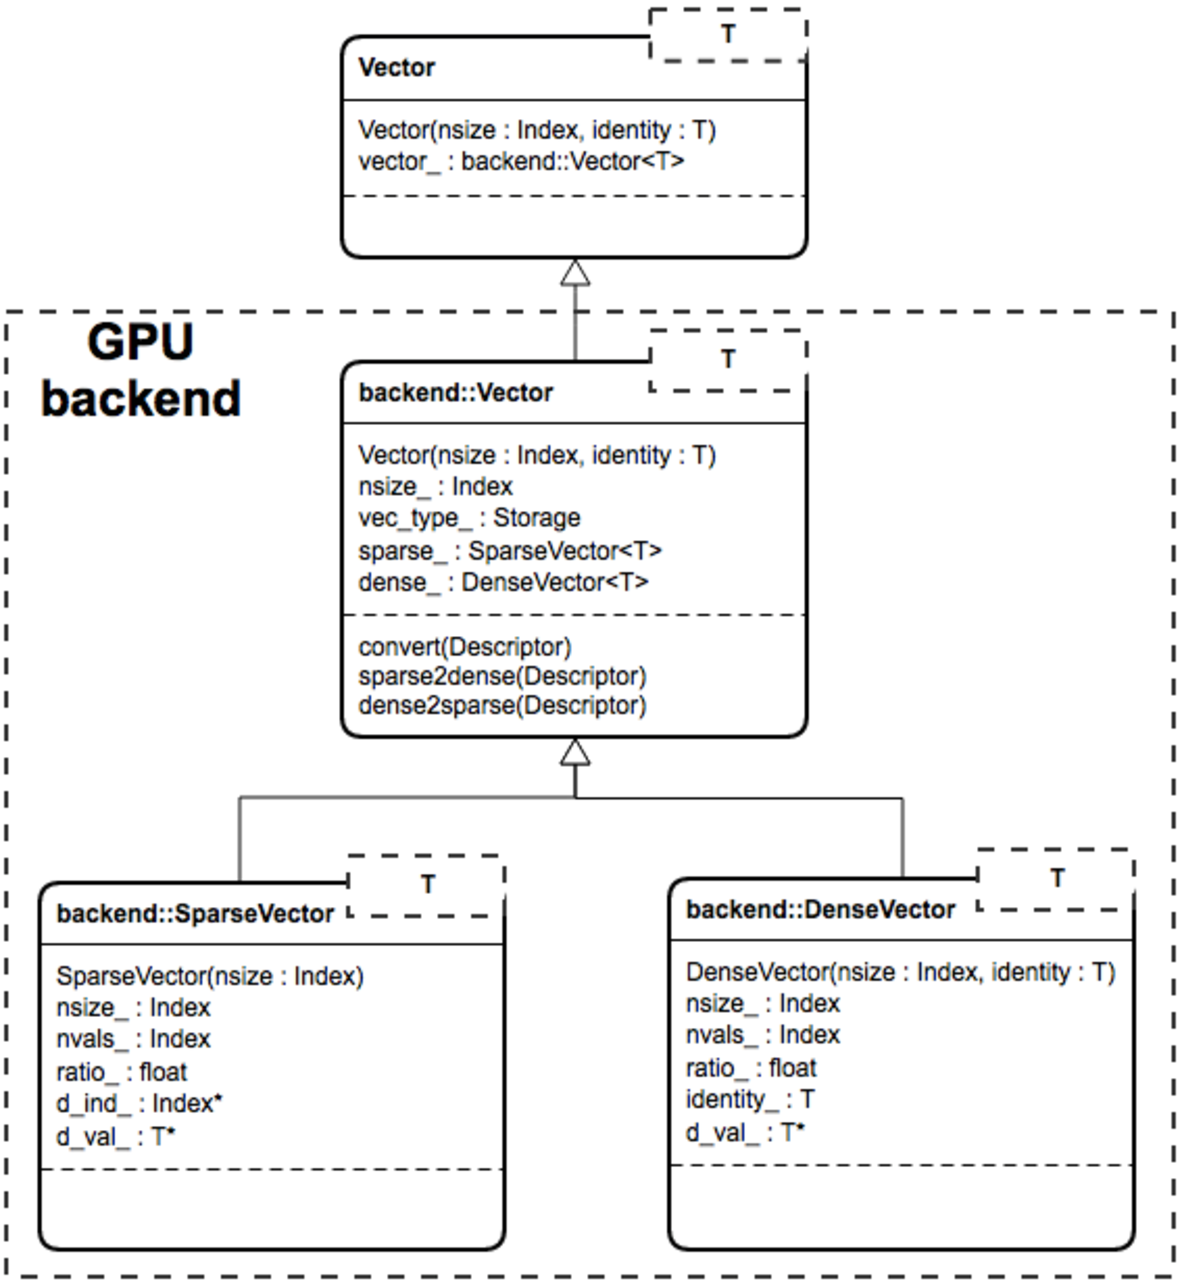
\includegraphics[width=\linewidth]{fig/graphblast}
	\caption{\textbf{GraphBLAST Vector UML diagram.}\label{fig:graphblast}}
\end{figure}

Direction-optimization is a good example where the power of abstracting away implementation details shines through, and the linear algebraic approach to graph analytics is at its most powerful. The end user has two conflicting desires:

\begin{enumerate}
	\item They want to communicate their request \emph{abstractly} enough that they do not have to decide whether the matrix-vector multiply is implemented as push, pull or any of the myriad possible ways.
	\item They want their computation to be described \emph{specifically} enough that the computer can optimize for the best approach for doing the computation.
\end{enumerate}

This desire is met by \verb'GrB_mxv', which is at the same time \emph{abstract} enough to not limit the computer in choosing push traversal when it should be choosing pull traversal, yet \emph{specific} enough that the computer has enough information to cut corners and pick the best algorithm.

Table~\ref{tab:loc} shows a comparison of how many lines of code it takes an implementation of GraphBLAS to express a given algorithm in C++. It is compared with two state-of-the-art graph frameworks in shared memory, the aforementioned Ligra~\cite{Shun:2013:Ligra} and GraphIt~\cite{Zhang:2018:GHP}, which is a DSL (domain specific language) designed for expressing graph algorithms.

\begin{table}[t]
	\centering
	\begin{tabular}{lccc}
		\toprule
		Algorithm      & Ligra~\cite{Shun:2013:Ligra} & GraphIt~\cite{Zhang:2018:GHP} & GraphBLAS  \\ \midrule
		Breadth-first-search & 29 & 22  & 25 \\
		Single-source shortest-path   & 55 & 25 & 25 \\
		Local graph clustering  & 84 & N/A  & 45 \\ \bottomrule
	\end{tabular}
	\caption{Comparison of lines of C++ application code counted by `cloc' except for numbers of GraphIt, which come from the paper~\cite{Zhang:2018:GHP}. N/A means not implemented. The specific GraphBLAS implementation for this comparison is GraphBLAST~\cite{Yang:2019:GBL}.\label{tab:loc}}
		%\vspace{-2em}
\hrule
\end{table}


